%! alt Three circles touch in pairs at D, E and F, with D at the top between the two equal circles of radius 25/6 centred at O2 and O3, and E and F on the large circle of radius 75/7 centred at O1. Triangle DEF has DE = DF = 5 and EF = 6. A dashed circle through D, E and F, centred at I with radius 25/8, is the incircle of the dashed triangle O1O2O3 of centres, touching its sides at D, E and F.
%! after_paragraph 1
%! scale 1/2
% The shared preamble of every Cevian figure. pipeline/figures turns these colours into theme-aware paint,
% and refuses any other colour, so draw only with them:
%   figink (lines and labels), figaux (construction lines), figaccent (the object the argument turns on),
%   figtint and figaccenttint (light fills).
\documentclass[border=1.5pt]{standalone}
\usepackage{tkz-euclide}
\definecolor{figink}{RGB}{0,0,0}
\definecolor{figaux}{RGB}{85,85,85}
\definecolor{figaccent}{RGB}{192,57,43}
\definecolor{figtint}{RGB}{221,221,221}
\definecolor{figaccenttint}{RGB}{245,213,208}
% tkz-euclide's defaults draw circles, compasses and marks in 50% grey and fill points with a tint.
\makeatletter
\def\tkz@otherlinecolor{figink}
\def\tkz@euc@circlecolor{figink}
\def\tkz@euc@compasscolor{figink}
\def\tkz@euc@mkcolor{figink}
\def\tkz@mk@fill{figink}
\def\tkz@euc@pointfillcolor{figink}
\makeatother
\tkzSetUpLine[color=figink,line width=.7pt]
\tkzSetUpArc[color=figink,line width=.7pt]
\tkzSetUpCompass[color=figink,line width=.5pt]
\tkzSetUpPoint[color=figink,fill=figink,size=3.1pt]
\tikzset{
  every picture/.style={line cap=round,line join=round,color=figink},
  circle style/.append style={color=figink,line width=.7pt},
  aux/.style={color=figaux,line width=.45pt,dash pattern=on 2.6pt off 2pt},
  key/.style={color=figaccent,line width=1pt},
  mk/.style={color=figink,line width=.5pt},
  lbl/.style={color=figink,inner sep=2.2pt},
  len/.style={color=figink,inner sep=1.5pt,font=\small},
}

\begin{document}
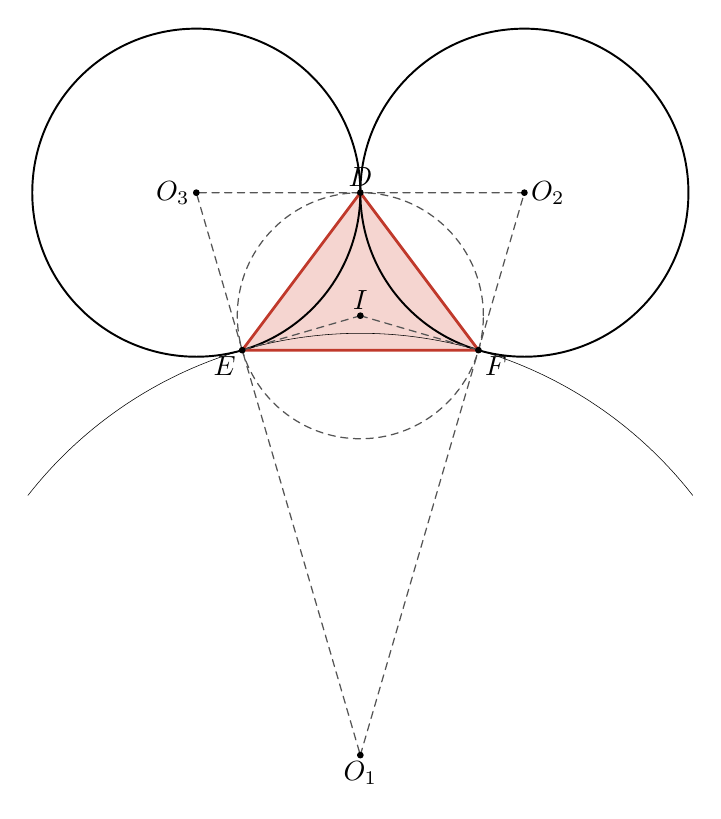
\begin{tikzpicture}
\tkzDefPoint(0.0,0.0){I} %! I = (0, 0)
\tkzDefPoint(0.0,1.5625000){D} %! D = (0, 25/8)
\tkzDefPoint(-1.5000000,-0.43750000){E} %! E = (-3, -7/8)
\tkzDefPoint(1.5000000,-0.43750000){F} %! F = (3, -7/8)
\tkzDefPoint(0.0,-5.5803571){O1} %! O1 = (0, -625/56)
\tkzDefPoint(4.2214862,-2.2821707){X} %! X = polar(O1, 75/7, 38)
\tkzDefPoint(-4.2214862,-2.2821707){Y} %! Y = polar(O1, 75/7, 142)
\tkzDefPoint(2.0833333,1.5625000){O2} %! O2 = (25/6, 25/8)
\tkzDefPoint(-2.0833333,1.5625000){O3} %! O3 = (-25/6, 25/8)
%! fact dist(D, E) == 5
%! fact dist(D, F) == 5
%! fact dist(E, F) == 6
%! fact dist(I, D) == 25/8
%! fact dist(I, E) == 25/8
%! fact dist(I, F) == 25/8
%! fact dist(O1, E) == 75/7
%! fact dist(O1, F) == 75/7
%! fact dist(O2, D) == 25/6
%! fact dist(O2, F) == 25/6
%! fact dist(O3, D) == 25/6
%! fact dist(O3, E) == 25/6
%! fact on_segment(F, O1, O2)
%! fact on_segment(E, O1, O3)
%! fact on_segment(D, O2, O3)
%! fact perp(O1, E, E, I)
%! fact perp(O1, F, F, I)
%! fact perp(O2, D, D, I)
%! fact tangent_circles(O1, 75/7, O2, 25/6)
%! fact tangent_circles(O1, 75/7, O3, 25/6)
%! fact tangent_circles(O2, 25/6, O3, 25/6)
%! fact dist(O1, X) == 75/7
%! fact dist(O1, Y) == 75/7
\tkzFillPolygon[color=figaccenttint](D,E,F)
\tkzDrawArc(O1,X)(Y)
\tkzDrawCircle(O2,D)
\tkzDrawCircle(O3,D)
\tkzDrawPolygon[aux](O1,O2,O3)
\tkzDrawCircle[aux](I,D)
\tkzDrawPolygon[key](D,E,F)
\tkzDrawSegments[aux](I,E I,F)
\tkzDrawPoints(D,E,F,I,O1,O2,O3)
\tkzLabelPoint[above,lbl](D){$D$}
\tkzLabelPoint[below left,lbl](E){$E$}
\tkzLabelPoint[below right,lbl](F){$F$}
\tkzLabelPoint[above,lbl](I){$I$}
\tkzLabelPoint[below,lbl](O1){$O_1$}
\tkzLabelPoint[right,lbl](O2){$O_2$}
\tkzLabelPoint[left,lbl](O3){$O_3$}
\end{tikzpicture}
\end{document}
